% Font options: 10pm, 11pt, 12pt
% Align headings left instead of center: nocenter
\documentclass[xcolor=x11names,compress]{beamer}\usepackage[]{graphicx}\usepackage[]{color}
%% maxwidth is the original width if it is less than linewidth
%% otherwise use linewidth (to make sure the graphics do not exceed the margin)
\makeatletter
\def\maxwidth{ %
  \ifdim\Gin@nat@width>\linewidth
    \linewidth
  \else
    \Gin@nat@width
  \fi
}
\makeatother

\definecolor{fgcolor}{rgb}{0.345, 0.345, 0.345}
\newcommand{\hlnum}[1]{\textcolor[rgb]{0.686,0.059,0.569}{#1}}%
\newcommand{\hlstr}[1]{\textcolor[rgb]{0.192,0.494,0.8}{#1}}%
\newcommand{\hlcom}[1]{\textcolor[rgb]{0.678,0.584,0.686}{\textit{#1}}}%
\newcommand{\hlopt}[1]{\textcolor[rgb]{0,0,0}{#1}}%
\newcommand{\hlstd}[1]{\textcolor[rgb]{0.345,0.345,0.345}{#1}}%
\newcommand{\hlkwa}[1]{\textcolor[rgb]{0.161,0.373,0.58}{\textbf{#1}}}%
\newcommand{\hlkwb}[1]{\textcolor[rgb]{0.69,0.353,0.396}{#1}}%
\newcommand{\hlkwc}[1]{\textcolor[rgb]{0.333,0.667,0.333}{#1}}%
\newcommand{\hlkwd}[1]{\textcolor[rgb]{0.737,0.353,0.396}{\textbf{#1}}}%
\let\hlipl\hlkwb

\usepackage{framed}
\makeatletter
\newenvironment{kframe}{%
 \def\at@end@of@kframe{}%
 \ifinner\ifhmode%
  \def\at@end@of@kframe{\end{minipage}}%
  \begin{minipage}{\columnwidth}%
 \fi\fi%
 \def\FrameCommand##1{\hskip\@totalleftmargin \hskip-\fboxsep
 \colorbox{shadecolor}{##1}\hskip-\fboxsep
     % There is no \\@totalrightmargin, so:
     \hskip-\linewidth \hskip-\@totalleftmargin \hskip\columnwidth}%
 \MakeFramed {\advance\hsize-\width
   \@totalleftmargin\z@ \linewidth\hsize
   \@setminipage}}%
 {\par\unskip\endMakeFramed%
 \at@end@of@kframe}
\makeatother

\definecolor{shadecolor}{rgb}{.97, .97, .97}
\definecolor{messagecolor}{rgb}{0, 0, 0}
\definecolor{warningcolor}{rgb}{1, 0, 1}
\definecolor{errorcolor}{rgb}{1, 0, 0}
\newenvironment{knitrout}{}{} % an empty environment to be redefined in TeX

\usepackage{alltt}
%\documentclass[xcolor=x11names,compress,handout]{beamer}
\usepackage[]{graphicx}
\usepackage[]{color}
\usepackage{booktabs}
\usepackage{hyperref}
\usepackage{tikz}
\usepackage{multirow}
\usepackage{dcolumn}
\usepackage{bigstrut}
\usepackage{amsmath} 
\usepackage{xcolor,colortbl}
\usepackage{amssymb}
%\newcommand{\done}{\cellcolor{teal}#1}

%% Beamer Layout %%%%%%%%%%%%%%%%%%%%%%%%%%%%%%%%%%
\useoutertheme[subsection=false,shadow]{miniframes}
\useinnertheme{default}
\usefonttheme{serif}
\usepackage{Arev}
\usepackage{pdfpages}
\usepackage[normalem]{ulem}

\setbeamerfont{title like}{shape=\scshape}
\setbeamerfont{frametitle}{shape=\scshape, size=\normalsize}

\definecolor{dkblue}{RGB}{0,0,102}

\setbeamercolor*{lower separation line head}{bg=dkblue} 
\setbeamercolor*{normal text}{fg=black,bg=white} 
\setbeamercolor*{alerted text}{fg=red} 
\setbeamercolor*{example text}{fg=black} 
\setbeamercolor*{structure}{fg=black} 
 
\setbeamercolor*{palette tertiary}{fg=black,bg=black!10} 
\setbeamercolor*{palette quaternary}{fg=black,bg=black!10} 

\renewcommand{\(}{\begin{columns}}
\renewcommand{\)}{\end{columns}}
\newcommand{\<}[1]{\begin{column}{#1}}
\renewcommand{\>}{\end{column}}

\setbeamertemplate{navigation symbols}{} 
\setbeamertemplate{footline}[frame number]
\setbeamertemplate{caption}{\raggedright\insertcaption\par}

\setbeamersize{text margin left=5pt,text margin right=5pt}

%%%%%%%%%%%%%%%%%%%%%%%%%%%%%%%%%%%%%%%%%%%%%%%%%%




\title{Making Causal Critiques}
\subtitle{Day 1 - Deconstructing an Argument}
\author{Jonathan Phillips}
\IfFileExists{upquote.sty}{\usepackage{upquote}}{}
\begin{document}

\frame{\titlepage}

\section{Introduction}

\begin{frame}
\frametitle{Causal Critiques}
\begin{itemize}
\item Political science is about \textit{explaining} outcomes
\pause
\begin{itemize}
\item Do parliamentary systems last longer than presidential ones?
\pause
\item Does development lead to democracy?
\pause
\item Does democracy prevent war?
\pause
\item Did voters support President Trump because of jobs lost to immigration?
\end{itemize}
\end{itemize}

\end{frame}

\begin{frame}
\frametitle{Causal Critiques}
\begin{itemize}
\item What is a causal critique?
\pause
\end{itemize}
\begin{table}[htbp]
  \centering
    \begin{tabular}{|>{\raggedright}p{5cm}|p{5cm}|}
    \hline
    Do parliamentary systems last longer than presidential ones? & "No, Parliamentary systems last longer because they are in Europe, not because they are parliamentary" \pause \\
    \hline
    Does development lead to democracy? & "No, democracy causes development" \pause \\
    \hline
    Does democracy prevent war? & "Of course not, India and Pakistan were democracies and had a war in 1999" \pause \\
    \hline
    Did voters support President Trump because of jobs lost to immigration? & "Obviously not, jobs were lost to technological change" \\
    \hline
    \end{tabular}%
  \label{tab:addlabel}%
\end{table}%
\end{frame}

\begin{frame}
\frametitle{Causal Critiques}
\begin{itemize}
\item What is a causal critique?
\begin{itemize}
\item A comment at a seminar
\pause
\item A critique of a policy
\pause
\item A response as a journal referee
\pause
\item Advice to a friend
\pause
\item A worry about your \textit{own} research paper
\end{itemize}
\end{itemize}
\end{frame}

\section{Effective argument}

\begin{frame}
\frametitle{What makes an Argument Convincing?}
\begin{itemize}
\item  Explanation requires:
\begin{enumerate}
\item  Theory
\item  Evidence
\end{enumerate}
\end{itemize}
\end{frame}

\begin{frame}
\frametitle{What makes an Argument Convincing?}
\begin{itemize}
\item  You plug your laptop in but it does not charge
\pause
\item You wiggle all the wires a few times and it starts to charge
\pause
\item So we have a solution, but do we have an \textit{explanation} for why it stopped working?
\pause
\item No! We do not know if the laptop, the charger, the adapter or the socket is the problem. We do not have a \textit{theory} to support our solution
\pause
\item Next time the laptop fails to charge, our wiggling might not be enough and we won't know how to fix it
\end{itemize}
\end{frame}

\begin{frame}
\frametitle{What makes an Argument Convincing?}
\begin{itemize}
\item How would we make an argument to explain why the laptop did not charge?
\pause
\begin{itemize}
\item We might focus on checking if the socket is working (a \textbf{Hypothesis})
\pause
\item This hypothesis is backed by \textbf{theory} - that faulty electricity supply in the socket prevents the laptop from charging
\pause
\end{itemize}
\item What evidence can we gather to test the theory?
\pause
\begin{itemize}
\item Try connecting the laptop to a different socket
\pause
\item If the laptop charges, we have support for our theory (\textbf{evidence})
\pause
\item If the laptop does not charge, we have less support for our theory (\textbf{evidence})
\pause
\item Note we cannot \textit{reject} the theory - it may be that both sockets are broken
\pause
\end{itemize}
\item We can design other tests to check the laptop, charger, adapter etc. 
\end{itemize}
\end{frame}

\begin{frame}
\frametitle{What makes an Argument Convincing?}
\begin{itemize}
\item Some tests are more informative than others
\pause
\begin{itemize}
\item If your friend plugs their own laptop and charger into the socket and it charges fine, we can rule out the socket being a problem
\pause
\item But we still do not know if your own laptop or charger are the problem
\pause
\end{itemize}
\item We need to design tests that \textit{distinguish between} specific theories
\end{itemize}
\end{frame}

\begin{frame}
\frametitle{What makes an Argument Convincing?}
\begin{itemize}
\item Theory on its own is not enough
\begin{itemize}
\item There are always many possible reasons for any single outcome
\pause
\end{itemize}
\item Evidence on its own is not enough
\begin{itemize}
\item The same evidence can be consistent with many possible mechanisms
\pause
\end{itemize}
\item Explanation requires evidence that supports a \textit{specific} theory
\begin{itemize}
\item And rejects other theories
\end{itemize}
\end{itemize}
\end{frame}

\begin{frame}
\frametitle{What makes an Argument Convincing?}
\begin{itemize}
\item Types of Tests (Collier 2011):
\pause
\begin{enumerate}
\item \textbf{Straw-in-the-Wind test}: Can raise or lower support for a hypothesis, but not confirm or reject
\pause
\item \textbf{Hoop Test}: Can reject a hypothesis but not confirm
\pause
\item \textbf{Smoking Gun Test}: Can confirm a hypothesis but not reject
\pause
\item \textbf{Doubly Decisive Test}: Can confirm a hypothesis and reject all other hypotheses
\end{enumerate}
\end{itemize}
\end{frame}

\begin{frame}
\frametitle{What makes an Argument Convincing?}
\begin{itemize}
\item Returning to our laptop charger puzzle...
\begin{enumerate}
\item \textbf{Straw-in-the-Wind test}: If we turn the lights on to check if there is power to the building in general
\pause
\item \textbf{Hoop Test}: If we test the laptop in another in another socket to make sure it works
\pause
\item \textbf{Smoking Gun Test}: If we test the charger to see if it fails in another socket
\pause
\item \textbf{Doubly Decisive Test}: If we test the charger with an entirely new socket and laptop that we have checked work
\end{enumerate}
\end{itemize}
\end{frame}

\begin{frame}
\frametitle{What makes an Argument Convincing?}
\begin{itemize}
\item What caused the reduction in price variation in Kerala's fishing industry?
\item \textbf{Hypothesis:} The introduction of mobile phone service
\item \textbf{Theory:} Mobile phones allowed people to quickly share the price of fish in different villages, so fishermen got the best prices more consistently
\begin{itemize}
\item Jensen et al (2007)
\item A 'smoking gun' test
\end{itemize}
\end{itemize}
\end{frame}

\setbeamercolor{background canvas}{bg=}
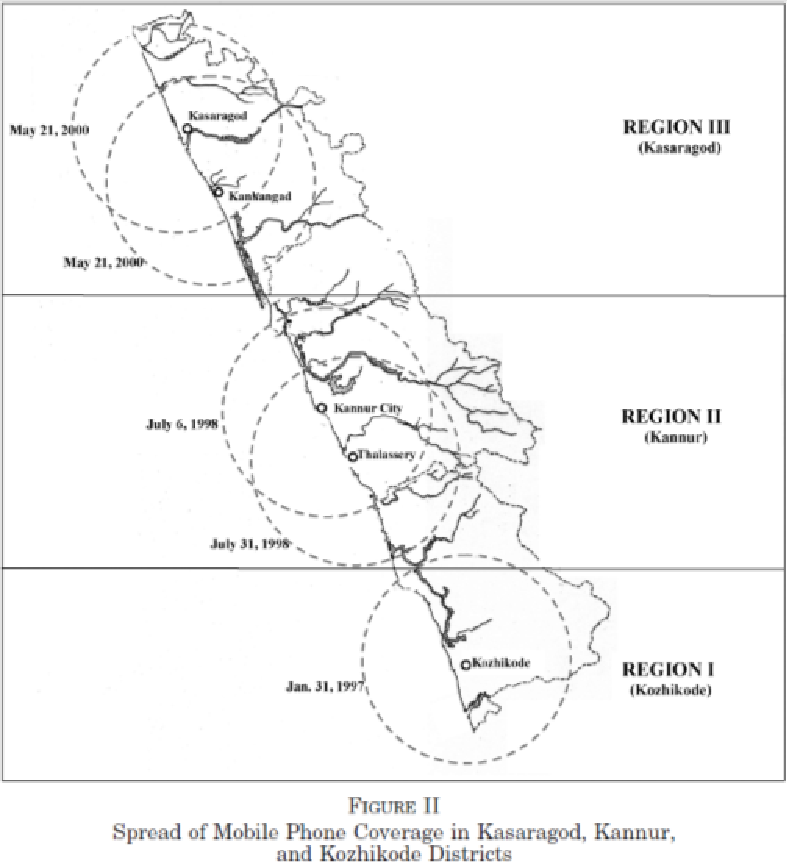
\includepdf[pages={1}]{Phone_Kerala.pdf}

\setbeamercolor{background canvas}{bg=}
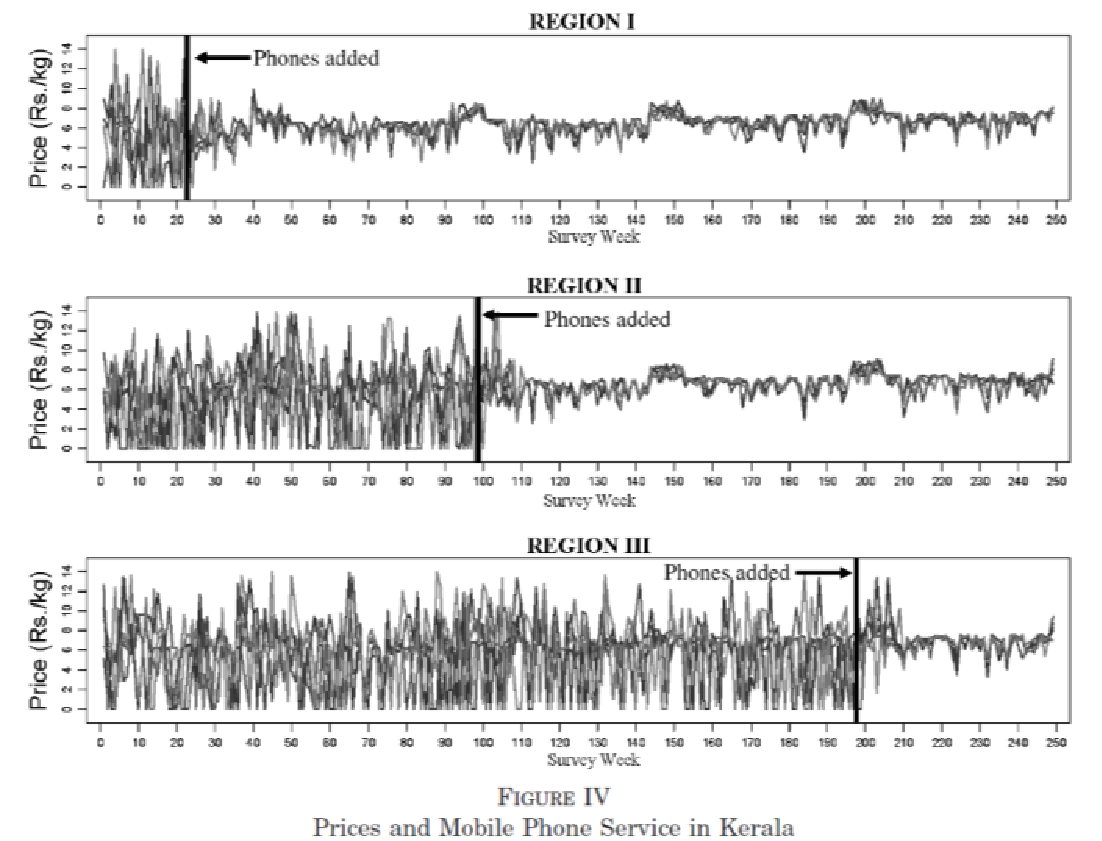
\includepdf[pages={1}]{Phone_Prices.pdf}

\begin{frame}
\frametitle{What makes an Argument Convincing?}
\begin{itemize}
\item Gathering evidence in political science is particularly hard:
\pause
\begin{enumerate}
\item Humans are complex and unpredictable, unlike the natural sciences
\pause
\item Societies are even more complex interactions of millions of humans
\pause
\item Everyone has an opinion, including researchers
\pause
\item Ethical constraints on the data we can gather
\pause
\item Political explanations in one place may not work in another
\end{enumerate}
\end{itemize}
\end{frame}

\begin{frame}
\frametitle{What makes an Argument Convincing?}
\begin{itemize}
\item Given the complexity of the real world, there are few causes which are \textbf{deterministic}
\pause
\item Most causes operate only if certain other hard-to-measure conditions are in place
\pause
\item That means we need to treat causation as \textbf{probabilistic}
\pause
\begin{itemize}
\item The presence of a cause does not guarantee an outcome
\item But raises the probability of an outcome
\pause
\end{itemize}
\item For example, a left-wing party in government may not guarantee the passage of social welfare legislation
\item But it can make it more likely
\end{itemize}
\end{frame}

\section{Consistent Theories}

\begin{frame}
\frametitle{Consistent Theories}
\begin{itemize}
\item To be good causal explanations, theories need to be \textbf{logically consistent}
\pause
\item Once we establish some premises, the conclusion should follow \textit{automatically}
\begin{itemize}
\item All policemen wear hats. This person is a policeman. Therefore this person is wearing a hat.
\pause
\item If it's true that all policemen wear hats and this person is a policeman, then it \textit{must} be true - by logic - that this person is wearing a hat
\pause
\item Formally: $\forall p:  h, p \Rightarrow h$
\end{itemize}
\end{itemize}
\end{frame}

\begin{frame}
\frametitle{Consistent Theories}
\begin{itemize}
\item Many explanations are \textbf{not} logically consistent:
\pause
\begin{itemize}
\item All policemen wear hats. This person is wearing a hat. Therefore this person is a policeman.
\pause
\item $\text{\sout{\ensuremath{\forall p:  h, \Rightarrow p}}}$
\item This is logically inconsistent
\end{itemize}
\end{itemize}
\end{frame}

\begin{frame}
\frametitle{Consistent Theories}
\begin{itemize}
\item Logical Fallacies
\pause
\begin{enumerate}
\item \textbf{False syllogism}: Conclusions do not follow from premises
\begin{itemize}
\item Eg. Some cats are black. Some black things are televisions. Therefore some cats are televisions.
\pause
\end{itemize}
\item \textbf{False dichotomy}: Restricting the possible options to only two
\begin{itemize}
\item Eg. "Either we attack them first or they attack us first"
\pause
\end{itemize}
\item \textbf{Circular reasoning}: The conclusions just restate the premises
\begin{itemize}
\item Eg. "Abortion should be legal because women have the right to an abortion."
\end{itemize}
\end{enumerate}
\end{itemize}
\end{frame}

\begin{frame}
\frametitle{Consistent Theories}
\begin{itemize}
\item Logical Fallacies
\pause
\begin{enumerate}
\setcounter{enumi}{3}
\item \textbf{Over-generalization}: Extending the conclusions beyond the scope of the evidence
\begin{itemize}
\item Eg. "All of my friends support party X so of course they will win the election"
\pause
\end{itemize}
\item \textbf{Post hoc Fallacy}: Just because something happened earlier does not mean it was the cause
\begin{itemize}
\item Eg. "You moved into this apartment yesterday and now the cooker is broken. It must be your fault."
\pause
\end{itemize}
\item \textbf{Appeal to Authority}: Assuming the author is right because they are senior
\begin{itemize}
\item Eg. Assuming that political science professors know what they are doing!
\end{itemize}
\end{enumerate}
\end{itemize}
\end{frame}

\begin{frame}
\frametitle{Consistent Theories}
\begin{itemize}
\item Logical Fallacies
\begin{enumerate}
\setcounter{enumi}{6}
\item \textbf{Fallacy of Composition}: Extending what is true of part to being true of the whole
\pause
\begin{itemize}
\item Eg. "If someone stands up at a football match, they can see better. Therefore, if everyone stands up, they can all see better."
\end{itemize}
\end{enumerate}
\end{itemize}
\end{frame}

\begin{frame}
\frametitle{Consistent Theories}
\begin{itemize}
\item Some political science arguments are logically inconsistent:
\begin{itemize}
\item Voters are rational - they choose the politician that is best for them. Therefore we always elect the best politicians.
\end{itemize}
\end{itemize}
\end{frame}

\section{Deconstructing Papers}

\begin{frame}
\frametitle{Deconstructing a Political Science Paper}
\begin{itemize}
\item How to read a political science paper:
\pause
\begin{itemize}
\item Actively, intentionally
\pause
\item Not like a Harry Potter book!
\pause
\item Read the abstract, conclusion, charts many times
\pause
\item Look for keywords: "We can conclude that...", "Our argument is that..."
\pause
\item Make notes \textit{only} of what you have learnt
\pause
\item Summarize the paper in your own words
\end{itemize}
\end{itemize}
\end{frame}

\begin{frame}
\frametitle{Deconstructing a Political Science Paper}
\begin{itemize}
\item Before we can critique an argument we have to understand its content
\pause
\begin{itemize}
\item What \textbf{concepts} it uses
\pause
\item How those concepts are \textbf{measured}
\pause
\item What \textbf{theory} connects the concepts
\pause
\item Where did the \textbf{evidence} (data) come from?
\pause
\item What \textbf{methodology} produced the evidence?
\pause
\item What is the \textbf{scope} of the argument's application?
\end{itemize}
\end{itemize}
\end{frame}

\begin{frame}
\frametitle{Deconstructing a Political Science Paper}
\begin{itemize}
\item Elements of a political science paper:
\pause
\begin{itemize}
\item \textbf{Research question} - the authors are engaging with a specific literature/puzzle
\pause
\item \textbf{Answer/Causal argument} - "We argue that D increases Y"
\pause
\item \textbf{Scope of argument} - Does the argument apply only to democracies, Asian countries, since World War II, only to women?
\end{itemize}
\end{itemize}
\end{frame}

\begin{frame}
\frametitle{Deconstructing a Political Science Paper}
\begin{itemize}
\item Elements of a political science paper:
\pause
\begin{itemize}
\item \textbf{Concepts/Variables} - What political factors do the authors think matter?
\pause
\item \textbf{Measures} - What factors do the authors actually measure?
\pause
\item \textbf{Units of Analysis} - At what level are these measures taken; individuals, countries, city-years?
\pause
\item \textbf{Role of Variables} - Which is the outcome variable and which the explanatory? What controls are used?
\end{itemize}
\end{itemize}
\end{frame}


\begin{frame}
\frametitle{Deconstructing a Political Science Paper}
\begin{itemize}
\item Elements of a political science paper:
\pause
\begin{itemize}
\item \textbf{Theory} - What social, economic or psychological process links the explanatory and outcome variables? 
\pause
\item \textbf{Methodology} - What strategy do the authors use to gather evidence to evaluate the theory?
\pause
\item \textbf{Evidence} - What evidence does the methodology produce?
\end{itemize}
\end{itemize}
\end{frame}

\setbeamercolor{background canvas}{bg=}
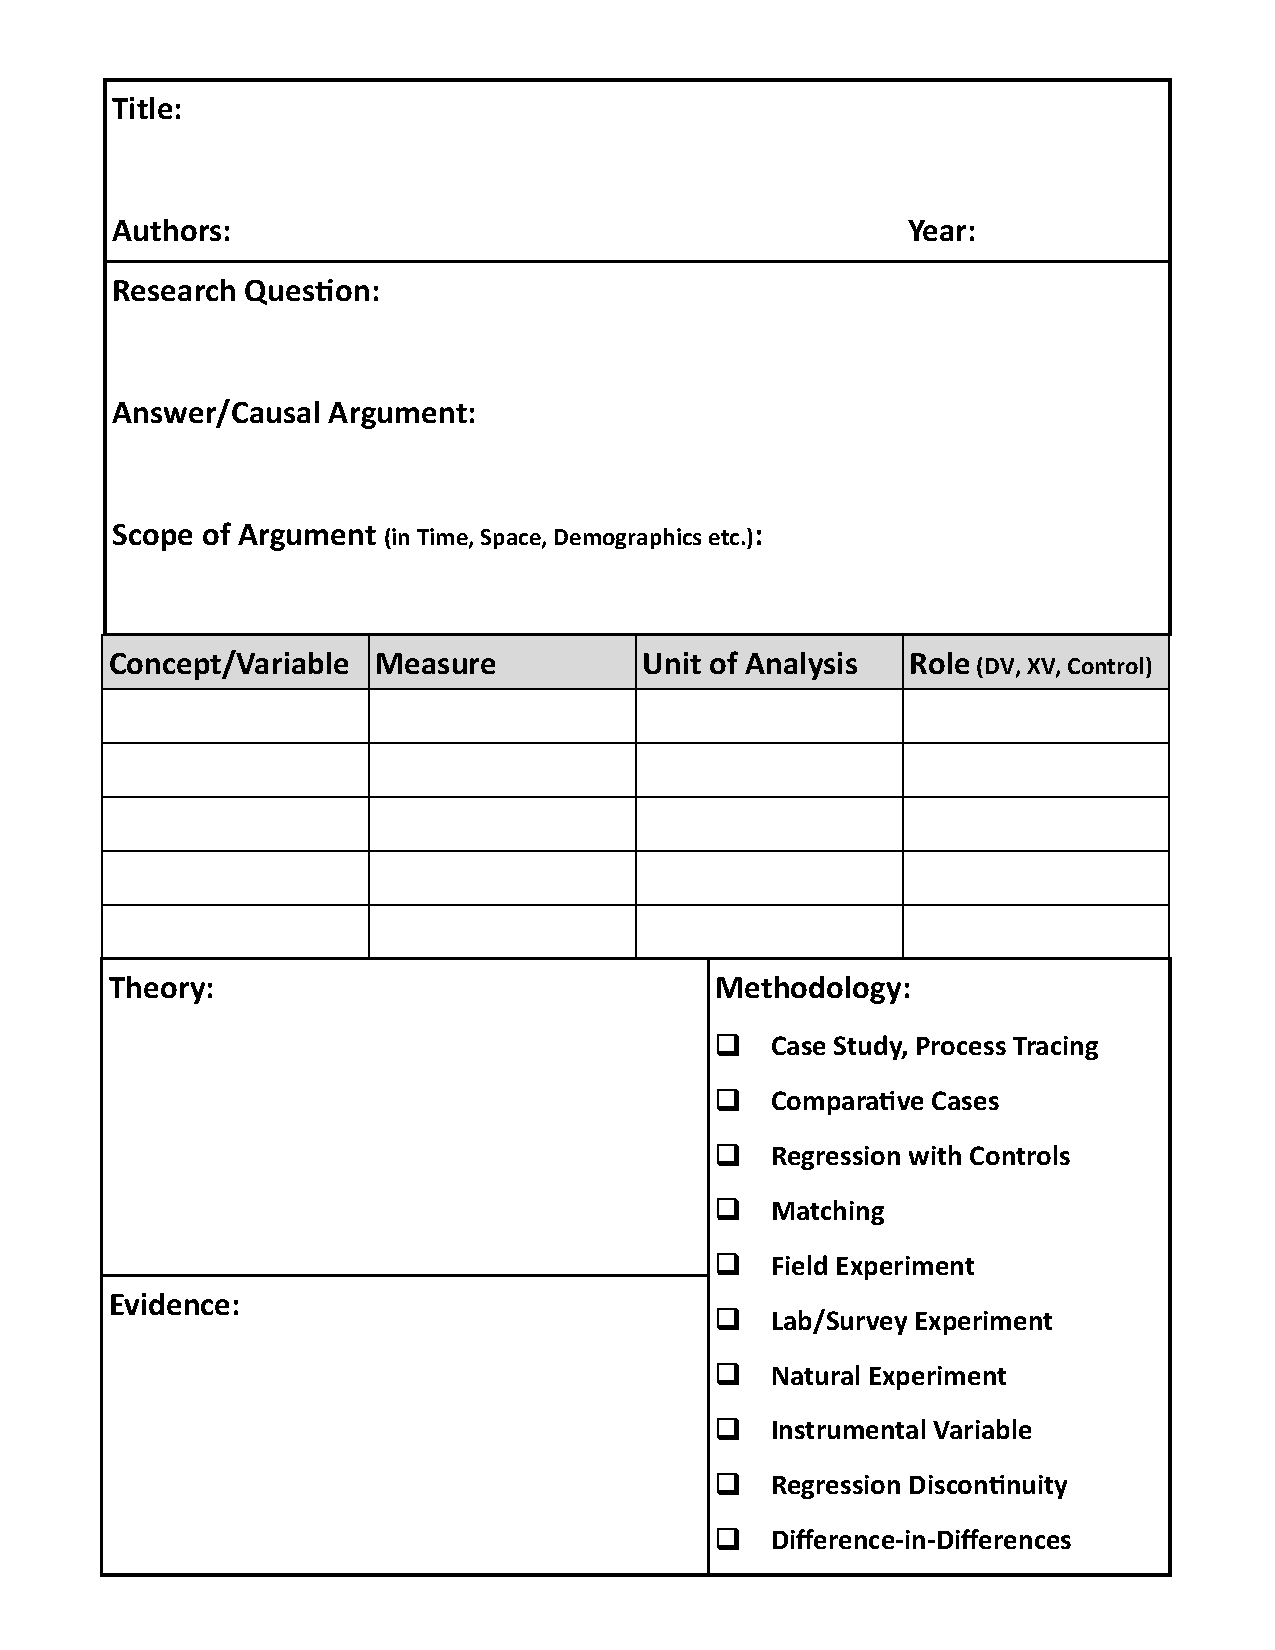
\includepdf[pages={1}]{Paper_summary_template.pdf}

\section{Fundamental Critiques}

\begin{frame}
\frametitle{Concepts and Measures}
\begin{itemize}
\item \textbf{Conceptual Validity} - Competitive authoritarianism vs. Illiberal Democracy
\pause
\begin{itemize}
\item Concepts must differentiate
\item But avoid conceptual stetching!
\pause
\item We can move "up and down the ladder of generality" (Sartori)
\item Eg. "competitive regimes" may not be democracies
\pause
\end{itemize}
\item \textbf{Measurement Validity} - when scores "meaningfully capture the ideas contained in the corresponding concept"
\pause
\begin{itemize}
\item Does the scale make sense? Is democracy binary or continuous?
\pause
\item Are the cases (units) scored correctly? How reliable is the scoring?
\end{itemize}
\end{itemize}
\end{frame}

\setbeamercolor{background canvas}{bg=}
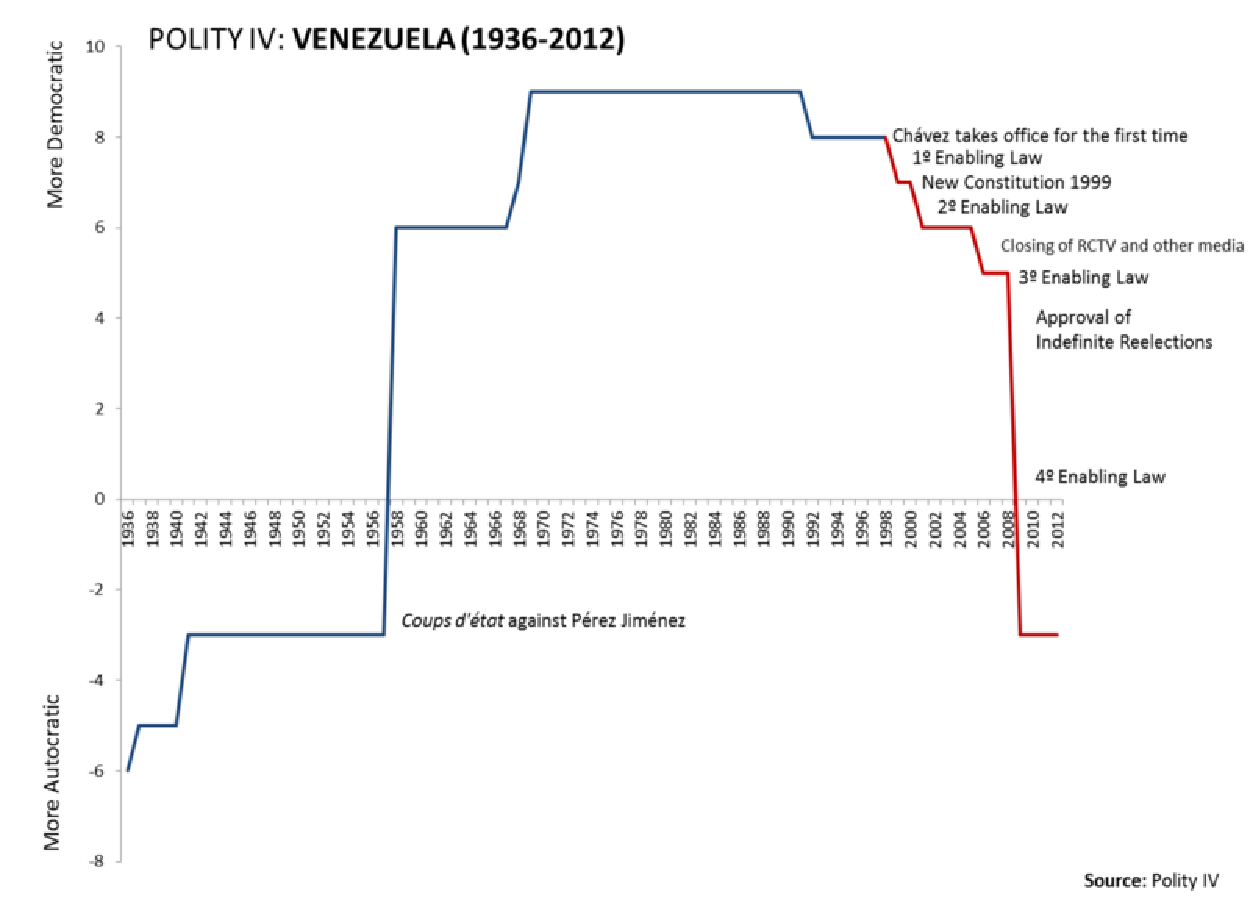
\includepdf[pages={1}]{Polity.pdf}


\begin{frame}
\frametitle{Methodology}
\begin{itemize}
\item Where did the dataset come from?
\pause
\begin{itemize}
\item Sampling strategy
\pause
\item Questionnaire and survey protocol
\pause
\item Measurement error
\pause
\item Data entry, cleaning
\pause
\item Statistics/statistical model chosen
\pause
\end{itemize}
\item What was the "Data Generating Process"?
\item How does this data help us answer the question?
\end{itemize}
\end{frame}

\begin{frame}
\frametitle{Methodology}
\begin{itemize}
\item Methodologies for gathering evidence:
\pause
\item Observational Studies:
\begin{itemize}
\item Case Study, Process Tracing
\pause
\item Comparative Cases
\pause
\item Regression with controls
\pause
\item Matching
\end{itemize}
\end{itemize}
\end{frame}

\begin{frame}
\frametitle{Methodology}
\begin{itemize}
\item Methodologies for gathering evidence:
\pause
\item Experimental Studies:
\pause
\begin{itemize}
\item Field Experiment
\pause
\item Lab/Survey Experiment
\end{itemize}
\end{itemize}
\end{frame}

\begin{frame}
\frametitle{Methodology}
\begin{itemize}
\item Methodologies for gathering evidence:
\pause
\item Quasi-Experimental Studies:
\pause
\begin{itemize}
\item Natural Experiment
\pause
\item Instrumental Variable
\pause
\item Regression Discontinuity
\pause
\item Difference-in-Differences
\end{itemize}
\end{itemize}
\end{frame}

\setbeamercolor{background canvas}{bg=}
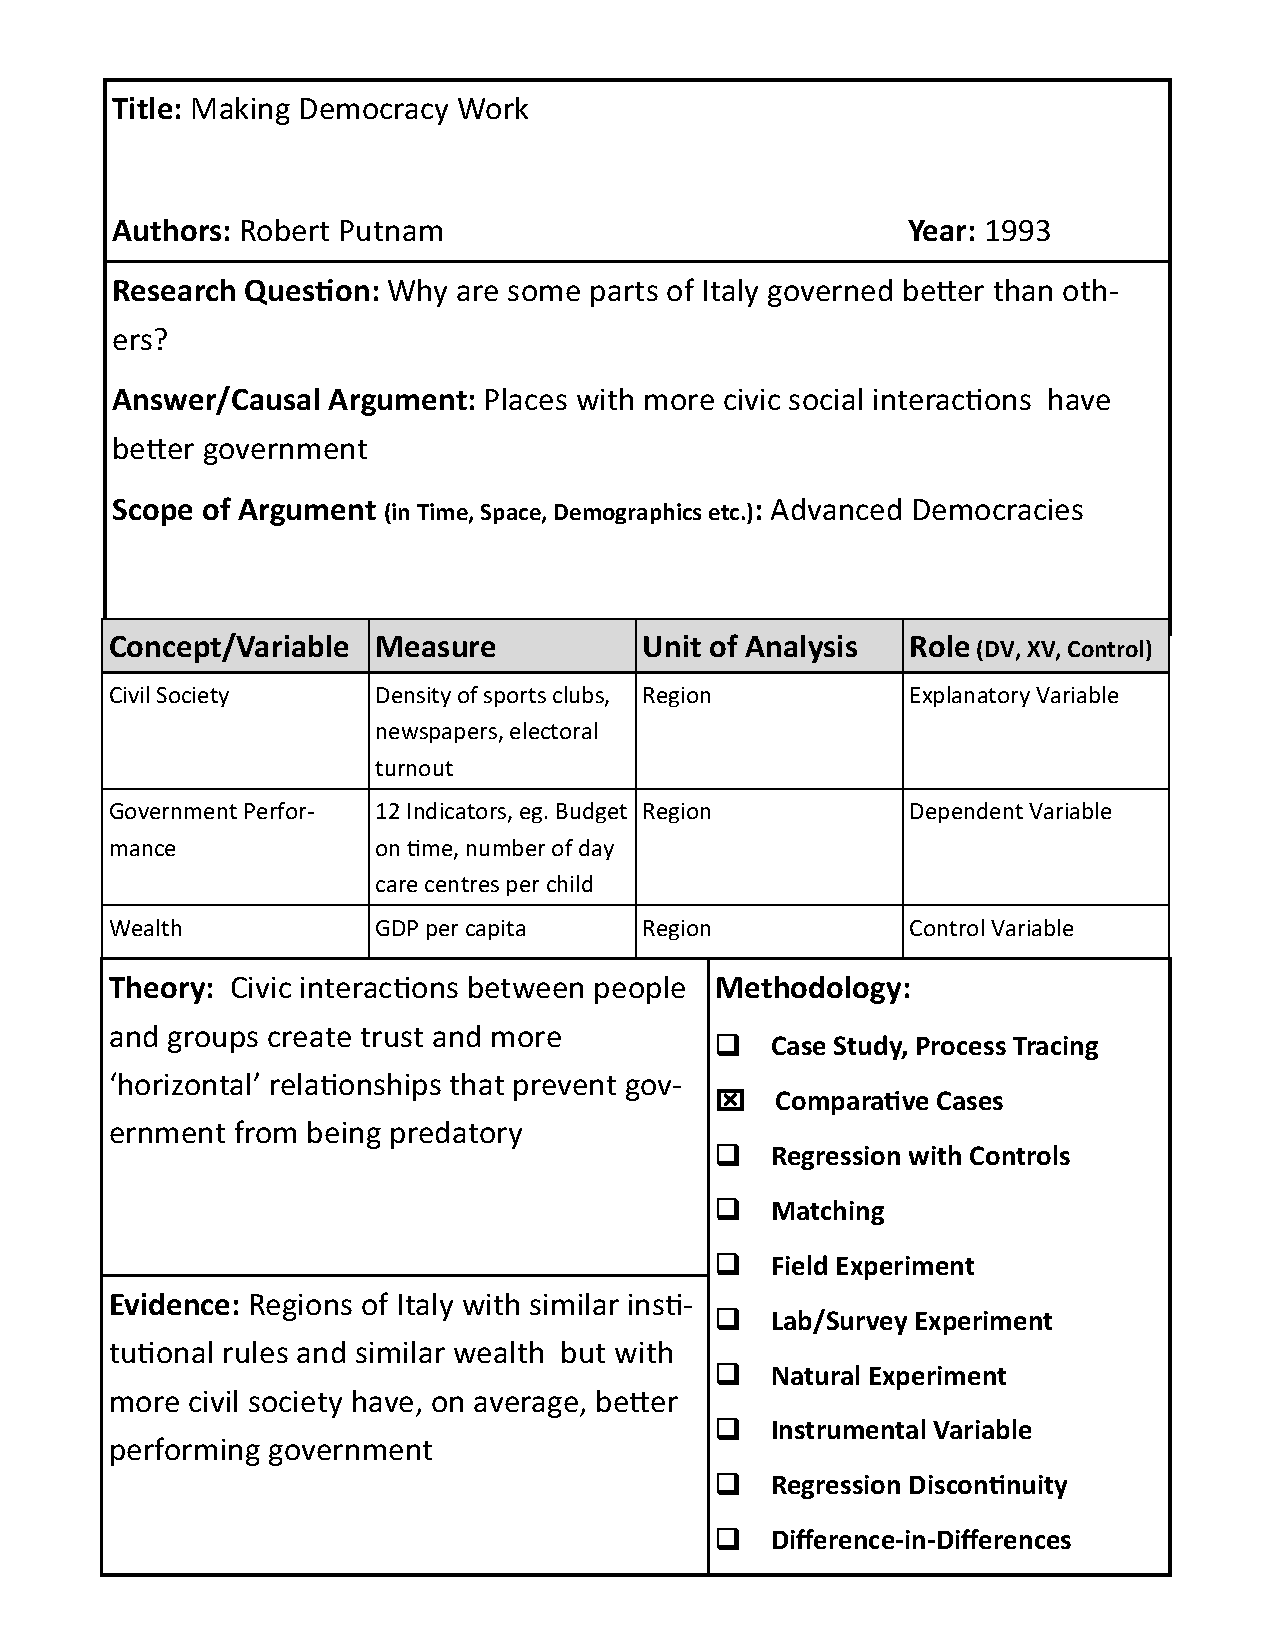
\includepdf[pages={1}]{Paper_summary_template_Putnam.pdf}

\begin{frame}
\frametitle{Causal Theory}
\begin{itemize}
\item Using Causal Diagrams to clarify arguments
\pause
\item Technically, "Directed Acyclical Graphs" (DAGs)
\pause
\begin{itemize}
\item Write all the variables on the paper
\pause
\item Connecting them with arrows to represent the author's \textbf{causal} argument
\pause
\item And also the \textit{threats} to the author's argument
\begin{itemize}
\item Even if they can't be measured
\end{itemize}
\end{itemize}
\end{itemize}
\end{frame}

\begin{frame}
\frametitle{Causal Theory}
\begin{knitrout}
\definecolor{shadecolor}{rgb}{0.969, 0.969, 0.969}\color{fgcolor}

{\centering 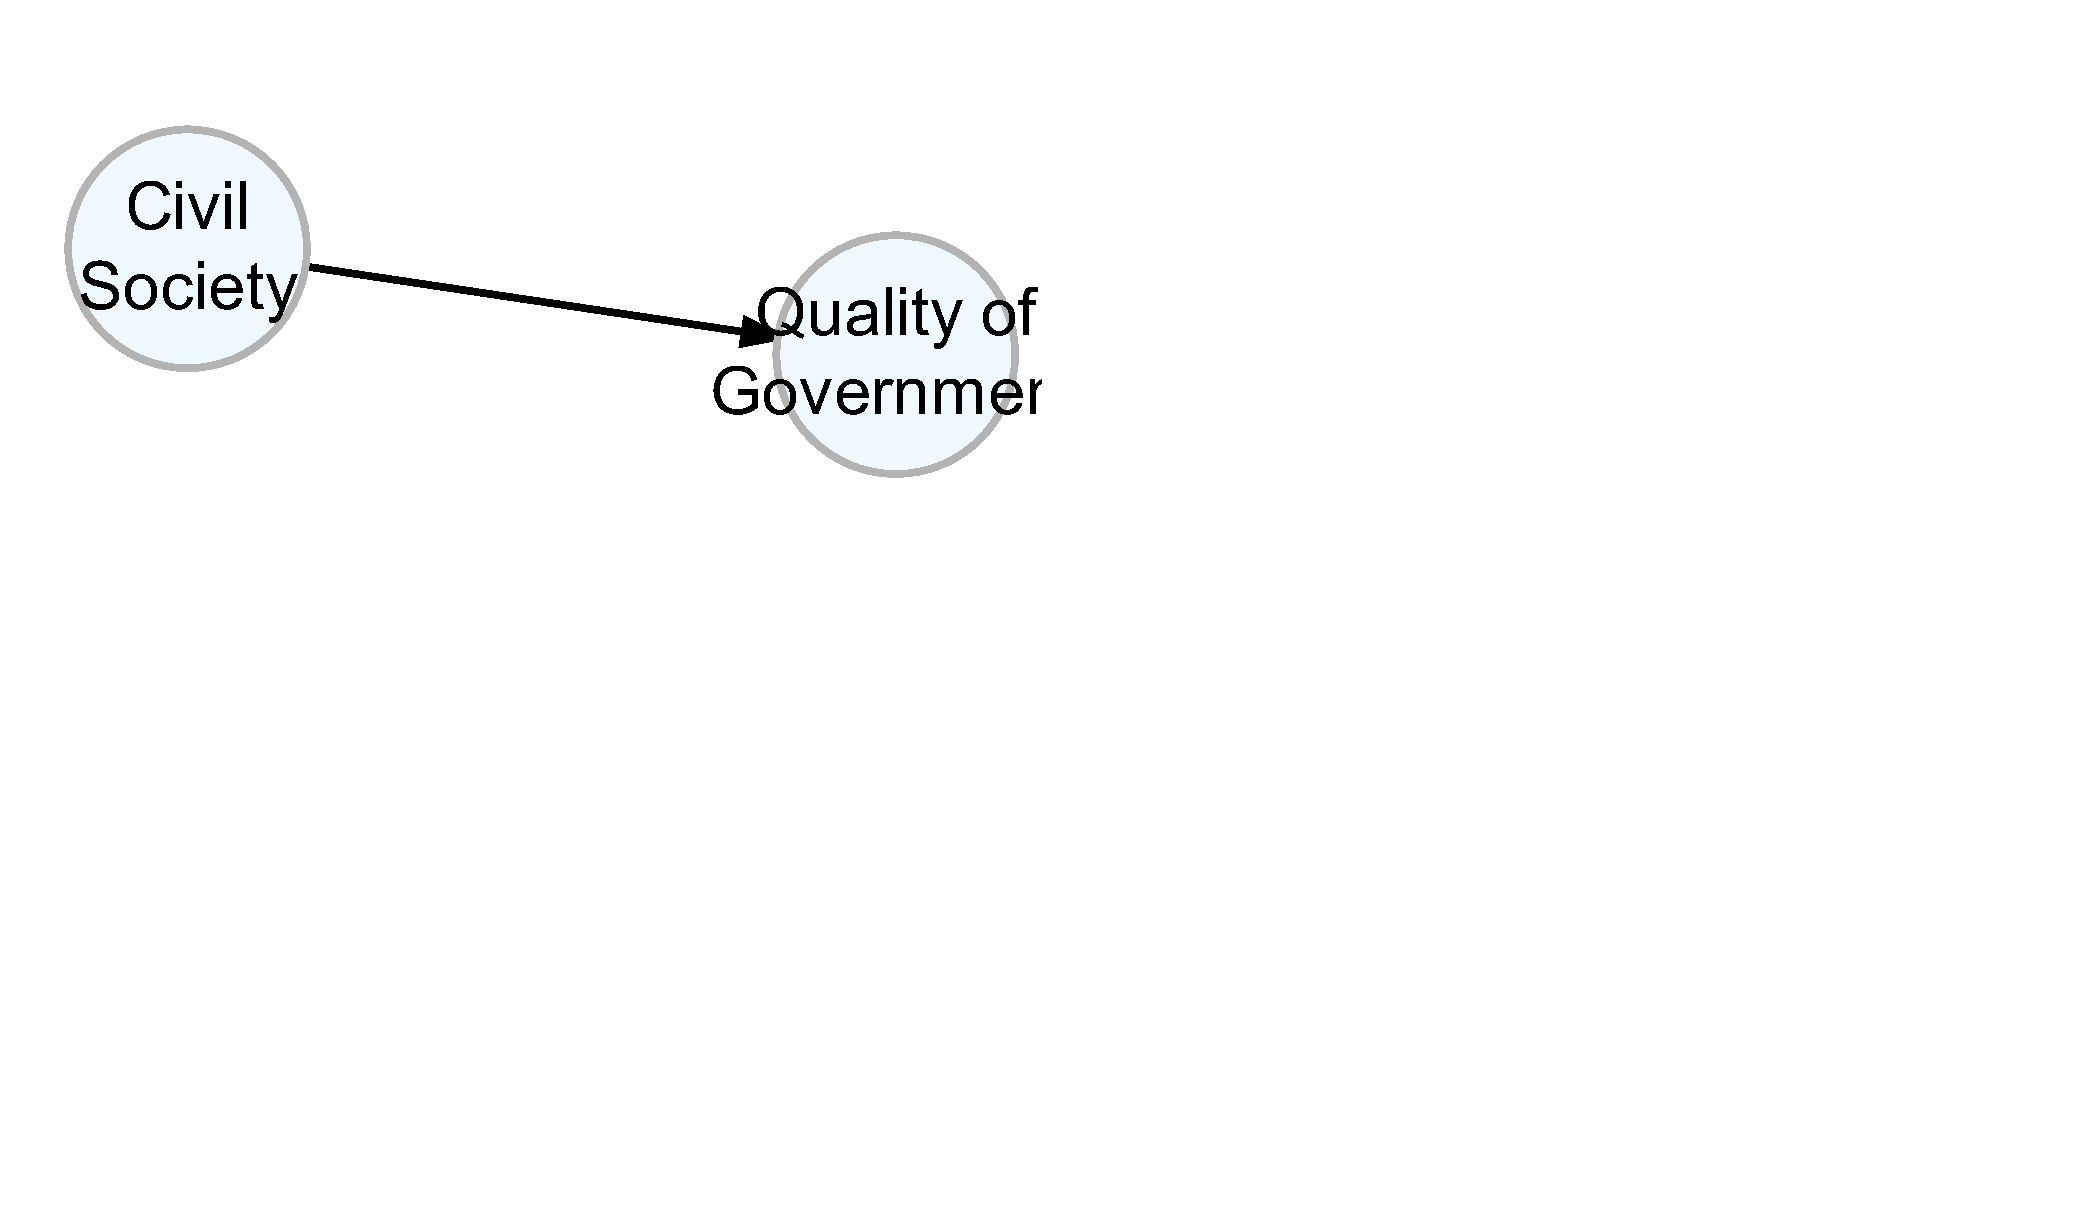
\includegraphics[width=\maxwidth]{figure/unnamed-chunk-1-1} 

}



\end{knitrout}
\end{frame}

\begin{frame}
\frametitle{Causal Theory}
\begin{knitrout}
\definecolor{shadecolor}{rgb}{0.969, 0.969, 0.969}\color{fgcolor}

{\centering 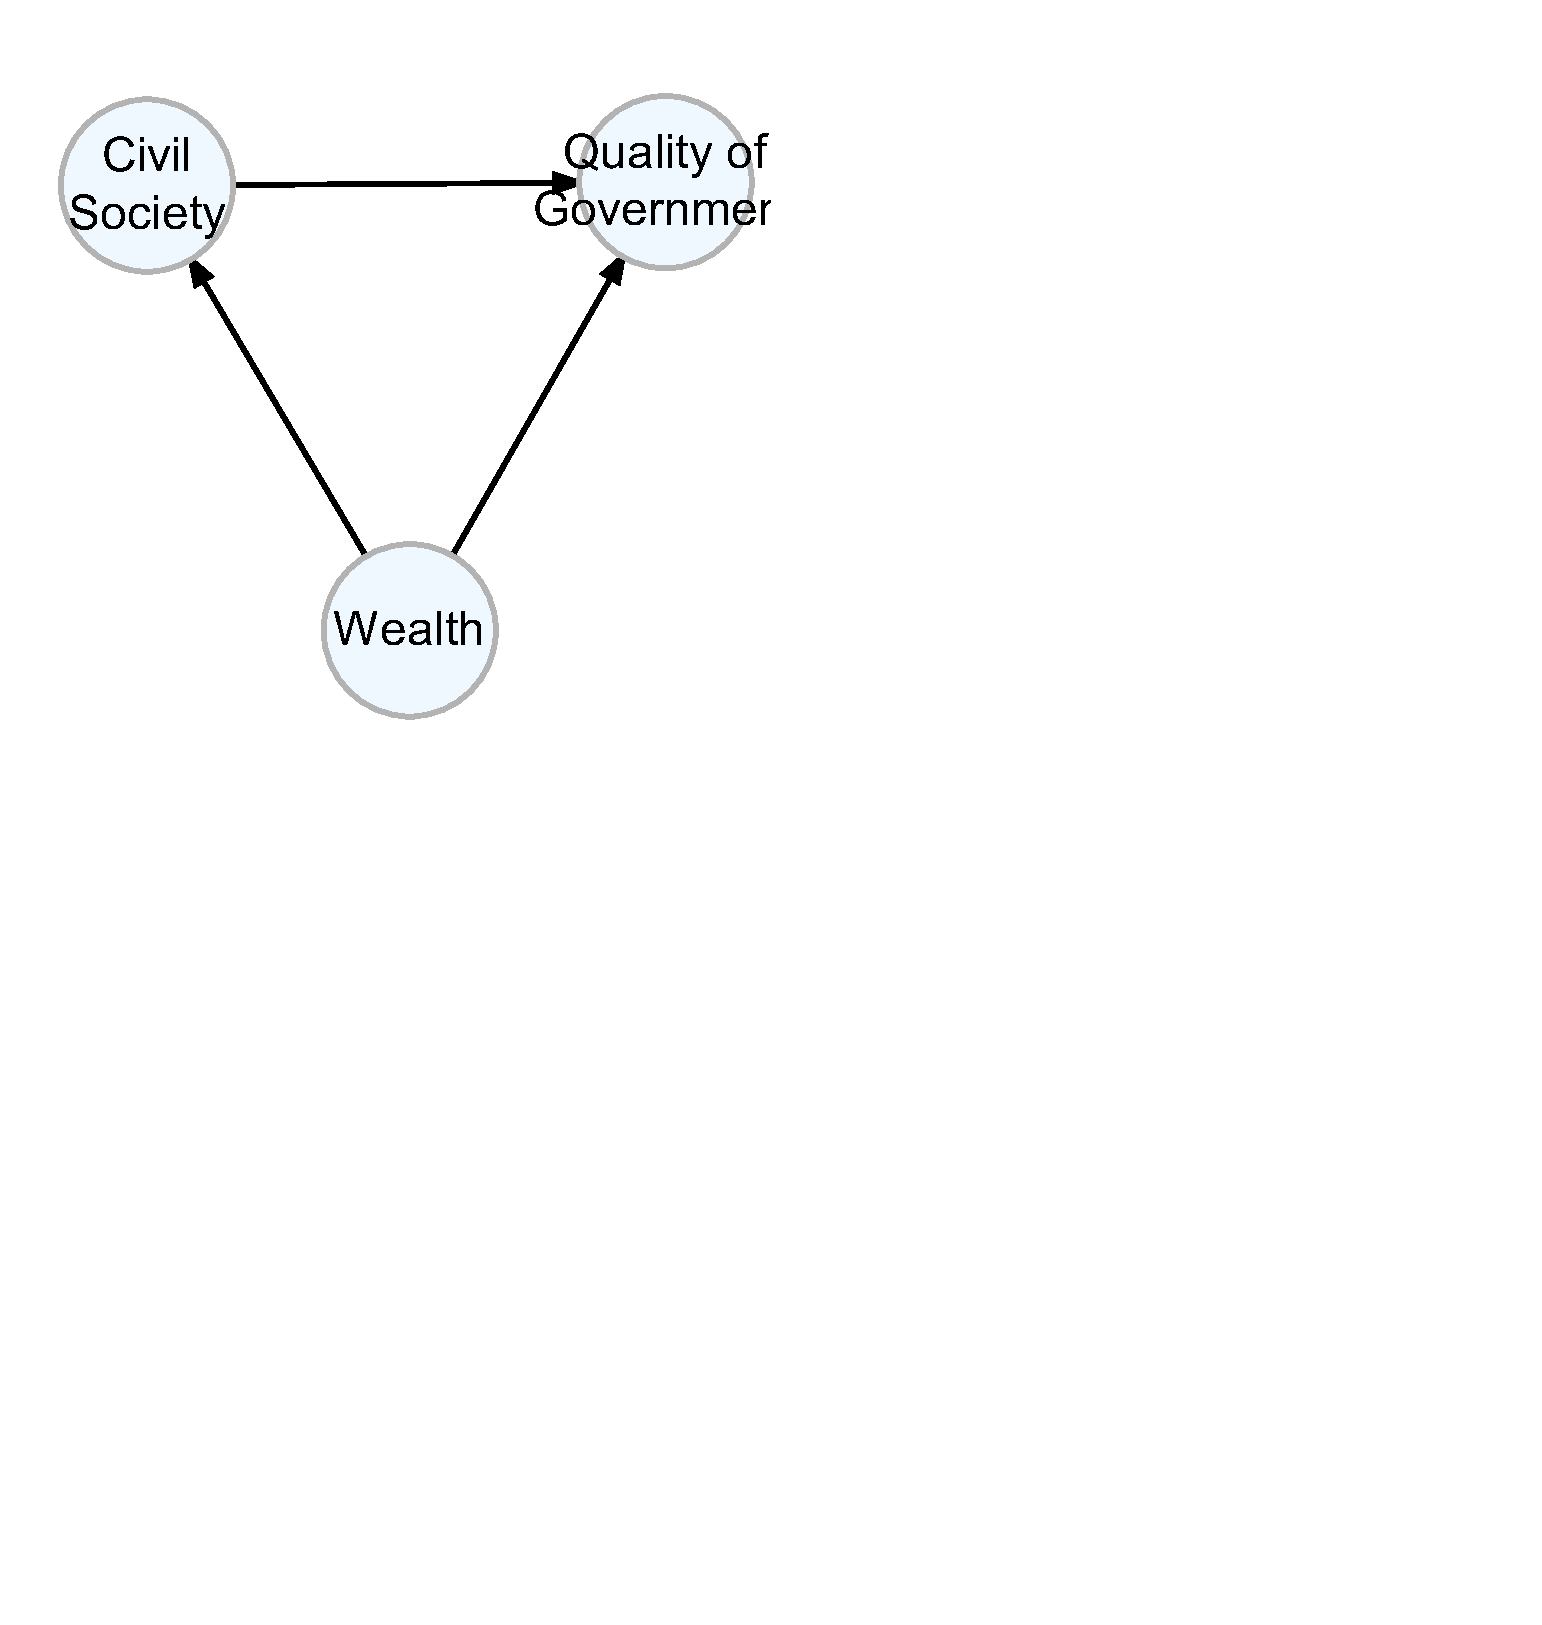
\includegraphics[width=\maxwidth]{figure/unnamed-chunk-2-1} 

}



\end{knitrout}
\end{frame}


\begin{frame}
\frametitle{Causal Theory}
\begin{knitrout}
\definecolor{shadecolor}{rgb}{0.969, 0.969, 0.969}\color{fgcolor}

{\centering 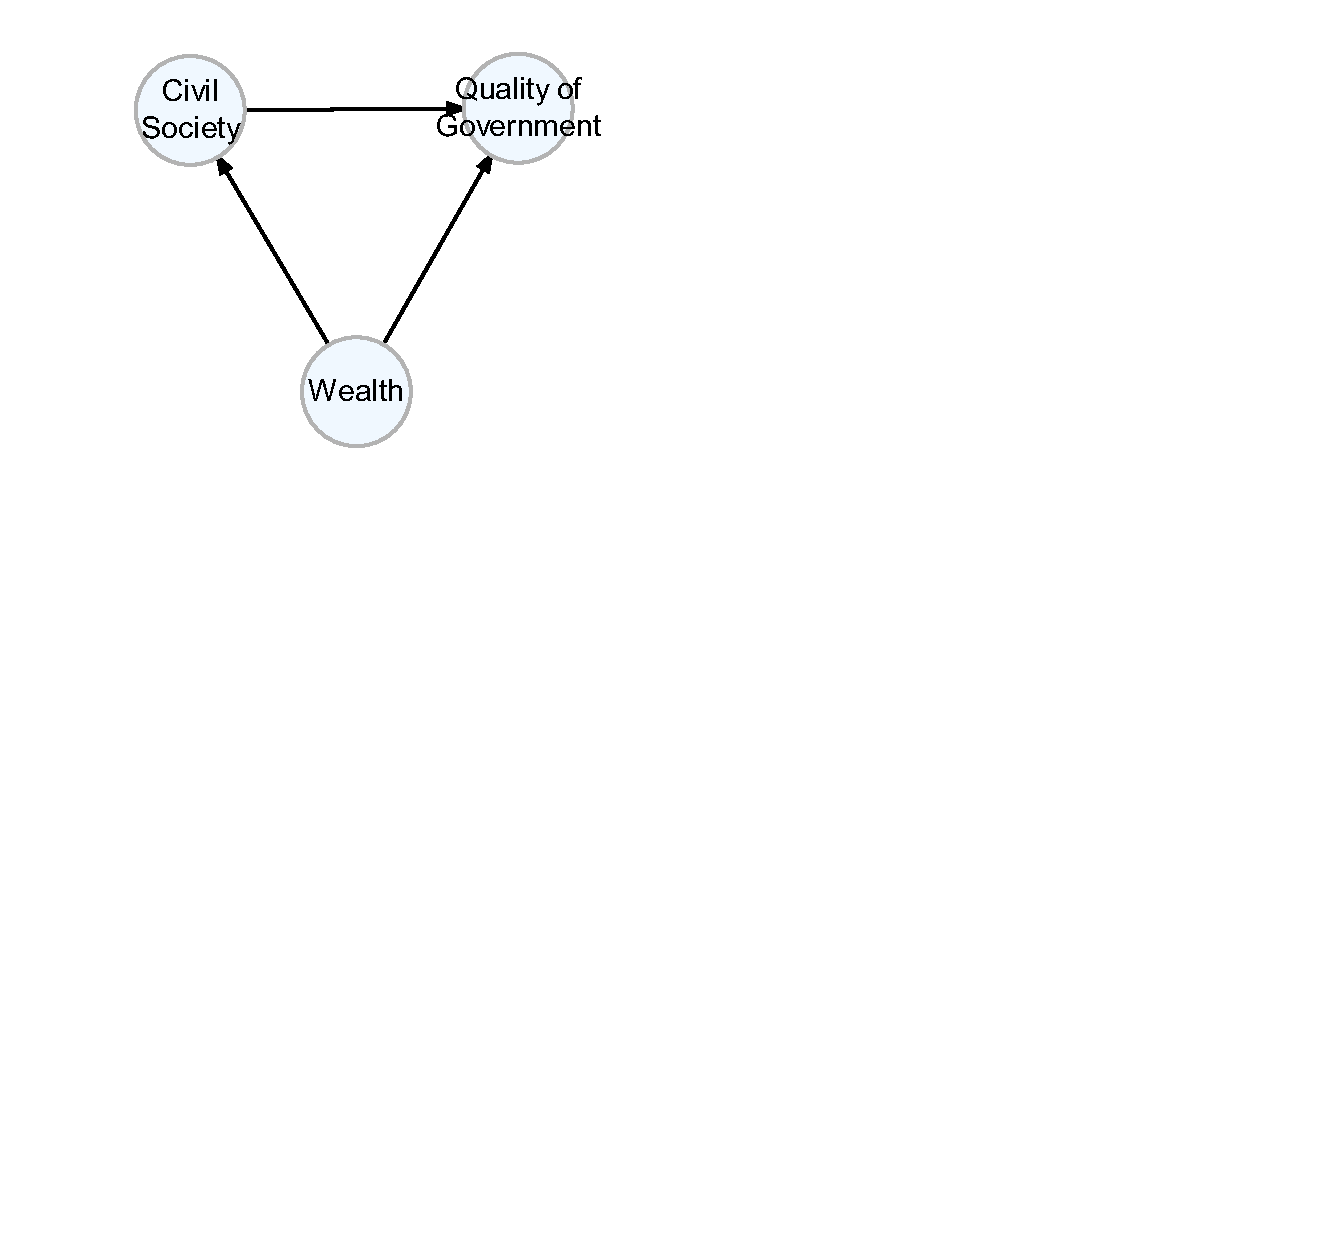
\includegraphics[width=\maxwidth]{figure/unnamed-chunk-3-1} 

}



\end{knitrout}
\end{frame}

\begin{frame}
\frametitle{Types of Causation}
\begin{enumerate}
\item \textbf{Deterministic Causation} - If $D$ then $Y$
\pause
\item \textbf{Probabilistic Causation} - If $D$ then the probability of $Y$ increases
\pause
\item \textbf{Conjuctural Causation} - If $D1$ and $D2$ then $Y$
\pause
\item \textbf{Equifinality Causation} - If $D1$ or $D2$ then $Y$
\pause
\item \textbf{Non-Linear Causation} - If $D>1000$ then $Y$
\pause
\item \textbf{Path-Dependent Causation} - If $D$ and $t=10$ then $Y$
\pause
\item \textbf{Granger Causation} - If $D$ causes $Y$, $D$ must be before $Y$
\end{enumerate}
\end{frame}


%%Types of Explanation

\begin{frame}
\frametitle{What makes a Good Causal Argument? (Gerring 2005)}
\begin{enumerate}
\item \textbf{Specificity} - Is the argument clear and internally consistent?
\pause
\item \textbf{Parsimony} - Is the argument simple?
\pause
\item \textbf{Power} - How much does $Y$ change?
\pause
\item \textbf{Precision} - How much uncertainty is there about how much $Y$ changes?
\pause
\item \textbf{Scope} - What is the breadth of conditions under which the effect occurs
\pause
\item \textbf{Differentiation} - Is the $D$ sufficiently different from the $Y$
\pause
\item \textbf{Normality} - Is $D$ a common event?
\pause
\item \textbf{Mechanism} - Do we understand what connects $D$ to $Y$?
\pause
\item \textbf{Consistency} - Is the argument consistent with our other knowledge about the rest of the world?
\pause
\item \textbf{Policy-relevance} - Can the argument help us design better policy?
\end{enumerate}
\end{frame}

\begin{frame}
\frametitle{What makes Good Causal Evidence? (Gerring 2005)}
\begin{enumerate}
\item \textbf{Sample Size} - How many cases are we learning from?
\pause
\item \textbf{Variation} - Do the causes and outcomes really vary in the sample?
\pause
\item \textbf{Representative} - Does the sample reflect the population?
\pause
\item \textbf{Independence} - Are the observations clustered (and therefore less useful)?
\pause
\item \textbf{Comparability} - Are the units of the same type?
\pause
\item \textbf{Transparency} - Do the data tell us about the mechanism connecting $D$ and $Y$?
\pause
\item \textbf{Replicability} - Can we take the same (or similar) data and reach the same conclusion?
\end{enumerate}
\end{frame}

\end{document}
 
 % effects of causes vs. reverse
